% Part   : Distribution
% Chapter: Anaconda Prompt
% Section: Identity
% ------------------------------------------------------------
% $Id$
% ------------------------------------------------------------

\begin{figure}[!hbp]
\hrulefill
\begin{verbatim}
trunk/Identity/Themes/$THEME/Distro/Anaconda/Prompt/
|-- img
|   |-- 3
|   |   |-- syslinux-splash-16c.png
|   |   |-- syslinux-splash-16c.pnm
|   |   |-- syslinux-splash.log
|   |   |-- syslinux-splash.lss
|   |   |-- syslinux-splash.png
|   |   |-- syslinux-splash.pnm
|   |   `-- syslinux-splash.ppm
|   |-- 4
|   |-- 5
|   `-- ... more major releases
|-- render.sh
`-- tpl
    `-- syslinux-splash.svg
\end{verbatim}
\hrulefill
\caption{Anaconda prompt identity's framework.%
   \label{fig:Distribution:Anaconda:Prompt:Identity}}
\end{figure}

\subsection{Designs Templates}
\hypertarget{sec:Distribution:Anaconda:Prompt:Identity:Templates}{}
\label{sec:Distribution:Anaconda:Prompt:Identity:Templates}

\begin{itemize}
\item trunk/Identity/Themes/\$THEME/Distro/Anaconda/Prompt/tpl
\end{itemize}

\subsection{Design Models}

\begin{itemize}
\item trunk/Identity/Models/Tpl/Distro/Anaconda/Prompt/
\item trunk/Identity/Models/Img/Distro/Anaconda/Prompt/
\end{itemize}

\begin{figure}[!hbp]
\begin{center}
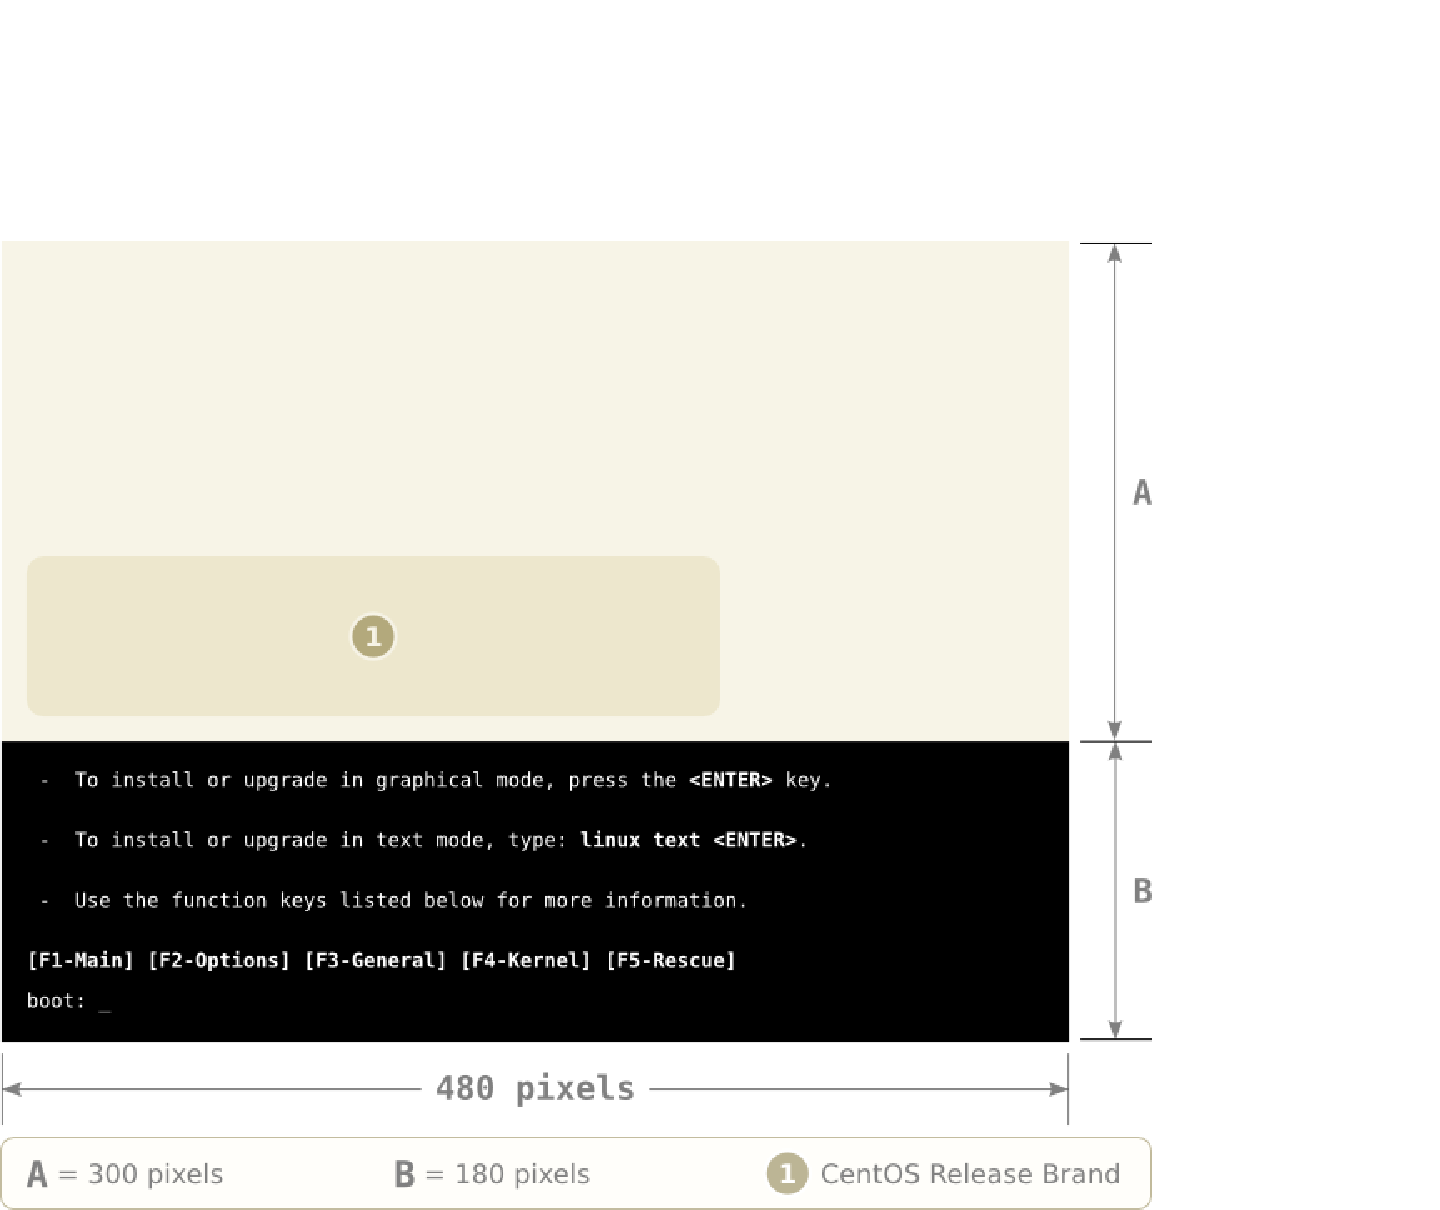
\includegraphics[width=0.8\textwidth]{%
    /home/centos/artwork/trunk/Identity/Models/Img/en/Distro/Anaconda/Prompt/syslinux-splash.pdf}
\end{center}
\caption{Anaconda prompt design model.% 
   \label{fig:Distribution:Anaconda:Model}}
\end{figure}

\begin{figure}[!hbp]
\begin{center}
\fbox{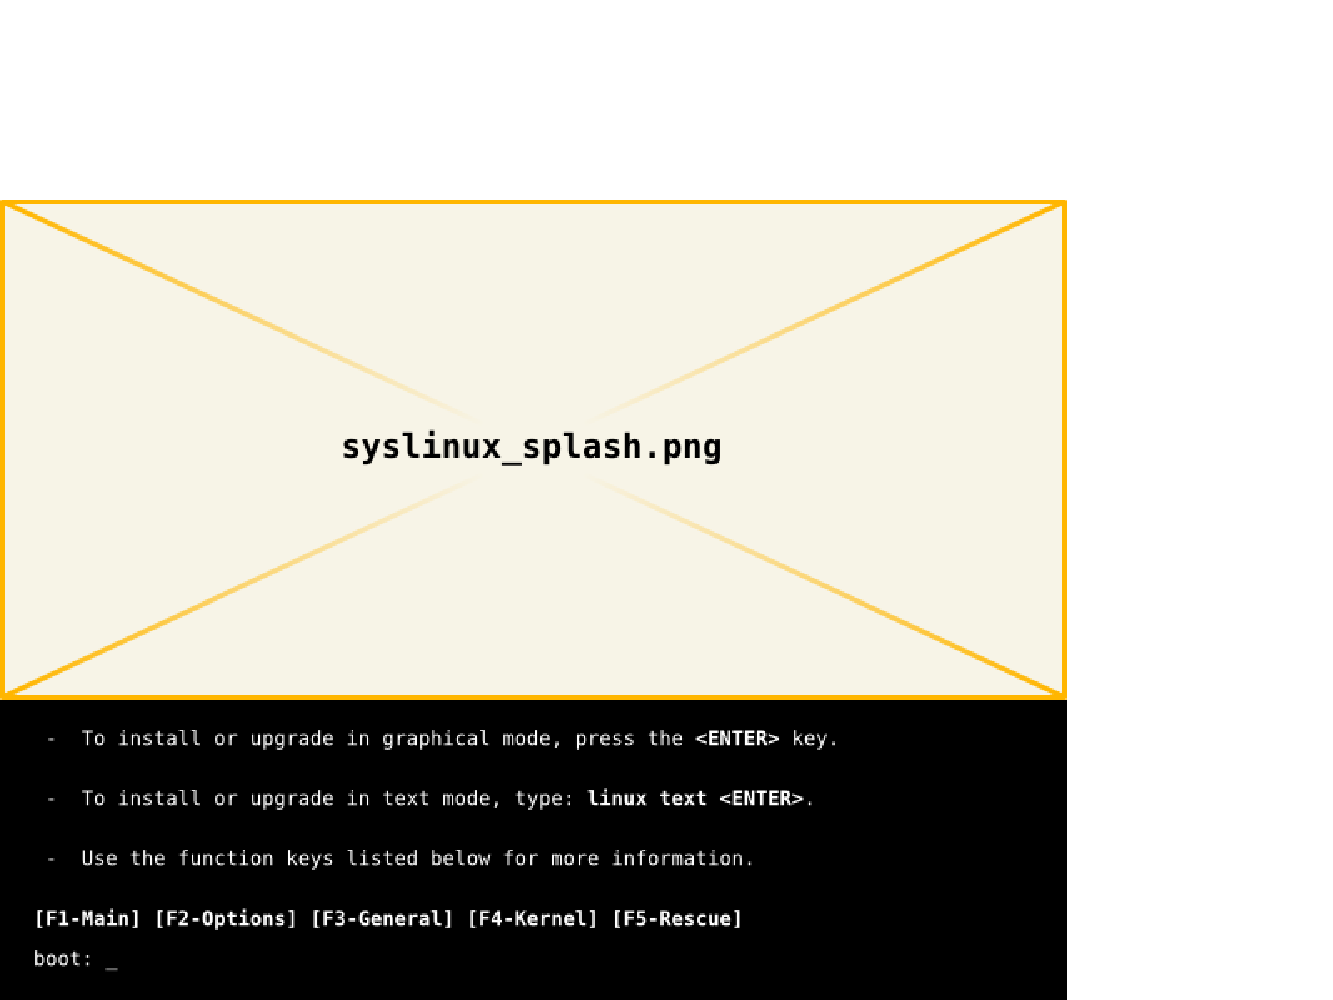
\includegraphics[width=0.8\textwidth]{%
   /home/centos/artwork/trunk/Identity/Models/Img/en/Distro/Anaconda/Prompt/fig-1-syslinux-splash.pdf}} 
\end{center}
\caption{Anaconda prompt position in the screen.% 
   \label{fig:Distribution:Anaconda:Prompt:Models:Fig2}}
\end{figure}

\subsection{Image Files}
\hypertarget{sec:Distribution:Anaconda:Prompt:Identity:Images}{}
\label{sec:Distribution:Anaconda:Prompt:Identity:Images}

\begin{itemize}
\item \texttt{syslinux-splash.png}: base image format.
\item \texttt{syslinux-splash.ppm}: auxiliar format.
\item \texttt{syslinux-splash.pnm}: auxiliar format.
\item \texttt{syslinux-splash.lss}: image format used by syslinux.
\item \texttt{syslinux-splash-16c.pnm}: 16 colors auxiliar format.
\item \texttt{syslinux-splash-16c.png}: 16 colors auxiliar format.
\item \texttt{syslinux-splash.log}: describes image convertion steps.
\end{itemize}

\subsection{Image Files Rendering}
\hypertarget{sec:Distribution:Anaconda:Prompt:Identity:Issues}{}
\label{sec:Distribution:Anaconda:Prompt:Identity:Issues}
\fbox{\texttt{./render.sh}}
\fbox{\texttt{./render.sh '5'}}
\fbox{\texttt{./render.sh '(3|4|5)'}}

\subsection{Color Limitations}
\hypertarget{sec:Distribution:Anaconda:Prompt:Identity:Colors}{}
\label{sec:Distribution:Anaconda:Prompt:Identity:Colors}

Anaconda Prompt does have color limitations. Initially, Anaconda
Prompt images are rendered without color limitation and later they are
indexed to 16 colors and converted to LSS16 format, as described in
\autoref{sec:Concepts:Identity:Themes:Palettes}. 

\subsection{Issues}
\hypertarget{sec:Distribution:Anaconda:Prompt:Issues}{}
\label{sec:Distribution:Anaconda:Prompt:Issues}

When creating Anaconda Prompt images some issues were found. They are
described below:

\begin{itemize}

\item \textbf{Many Different Colors:}

As more different colors you have on your design, more are the
possibilities of increasing the amount of noise in your design after
indexing to 16 colors. For example, if you include the actual CentOS
symbol in this image, it ocupies 3 colors (for the orange, green,
violet) in the indexed image which are completely different and
non-reusable in the blue toned background image.

\item \textbf{The CentOS Symbol:}

As previously said, if we include the CentOS default symbol in
Anaconda Prompt there is a color degradation and a reduction of
available colors to use in the 16 colors indexed image.

Some tests were made with variants of CentOS default symbol, but they
all were declined because they bring confusion about which is the
CentOS default symbol.

It would be very convenient to CentOS visual identity if the CentOS
default symbol could be included, \textit{exactly as it is}, in
Anaconda Prompt images.

\end{itemize}

